% Source ID: src-c47985c709ff8ae42e6e192879d604223c58a53c4358056d28f78ad5a9736e3c
% Source PDF SHA-256: a33455d27abdf2c4b344a5b90395bd71269f6fbefdef350375aba074e47ef700
% Source page 1 (printed page 943), question 17. Hidden edges and auxiliary segments follow the fixed page.
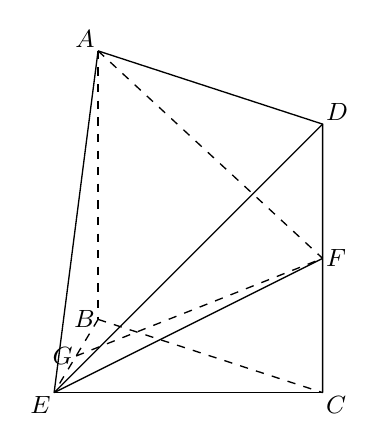
\begin{tikzpicture}[
  x=0.62cm,
  y=0.62cm,
  every node/.style={font=\small,inner sep=1pt},
  line width=0.48pt
]
\coordinate (A) at (0.9,7.0);
\coordinate (B) at (0.9,1.5);
\coordinate (C) at (5.5,0);
\coordinate (D) at (5.5,5.5);
\coordinate (E) at (0,0);
\coordinate (F) at (5.5,2.75);
\coordinate (G) at (0.45,0.75);

% Visible outline and construction segments.
\draw (A)--(D)--(C);
\draw (E)--(A);
\draw (E)--(C);
\draw (E)--(D);
\draw (E)--(F);
\draw[dashed] (A)--(B);
\draw[dashed] (B)--(C);
\draw[dashed] (B)--(E);
\draw[dashed] (A)--(F);
\draw[dashed] (G)--(F);

\node[above left] at (A) {$A$};
\node[left] at (B) {$B$};
\node[below right] at (C) {$C$};
\node[above right] at (D) {$D$};
\node[below left] at (E) {$E$};
\node[right] at (F) {$F$};
\node[left] at (G) {$G$};
\end{tikzpicture}
